\section{O Método Bootstrap}

\begin{frame}{O Princípio do Bootstrap}
    \begin{block}{Origem do Nome}
        Derivado da expressão \textit{"to pull oneself up by one's own bootstraps"} (erguer-se puxando as próprias botas). Remete a realizar uma tarefa impossível utilizando apenas os recursos disponíveis.
    \end{block}
    
    \begin{block}{Idéia Central}
        A amostra observada é a melhor representação disponível da população desconhecida. 
        Reamostrar \textbf{com reposição} dessa amostra imita o processo de retirar amostras da própria população original.
    \end{block}
\end{frame}

\begin{frame}{O Algoritmo do Bootstrap}
    \begin{enumerate}
        \item Considere uma amostra original $S$ de tamanho $N$.
        \item Crie uma nova amostra (reamostra bootstrap) sorteando $N$ elementos de $S$ \textbf{com reposição}.
        \item Calcule a estatística desejada (ex: média) para essa reamostra.
        \item Repita os passos 2 e 3 um número elevado de vezes (ex: $M = 5000$).
        \item Use a distribuição das estatísticas geradas para estimar variabilidade e limites de confiança.
    \end{enumerate}
\end{frame}

\begin{frame}{Exemplo Matemático: Bootstrap Manual}
    \begin{block}{Problema}
        Temos uma amostra inicial pequena $S = \{2, 4, 9\}$ com $N = 3$.
        A média observada é $\bar{X} = 5.0$.
        Vamos simular a amostragem com reposição para obter 4 reamostras bootstrap:
    \end{block}
    \begin{block}{Simulações de Reamostragem}
        \begin{itemize}
            \item \textbf{Reamostra 1:} $\{2, 2, 9\} \rightarrow \bar{X}^*_1 = \frac{13}{3} \approx 4.33$
            \item \textbf{Reamostra 2:} $\{4, 9, 9\} \rightarrow \bar{X}^*_2 = \frac{22}{3} \approx 7.33$
            \item \textbf{Reamostra 3:} $\{2, 4, 4\} \rightarrow \bar{X}^*_3 = \frac{10}{3} \approx 3.33$
            \item \textbf{Reamostra 4:} $\{9, 2, 9\} \rightarrow \bar{X}^*_4 = \frac{20}{3} \approx 6.67$
        \end{itemize}
        A distribuição das médias bootstrap obtida é $\{3.33, 4.33, 6.67, 7.33\}$.
        Em escala real, faríamos isso 5000 vezes para obter percentis estáveis.
    \end{block}
\end{frame}

\begin{frame}[fragile]{Demonstração em Python: Bootstrap Manual}
    \begin{lstlisting}[language=Python]
import numpy as np

# Amostra original
S = np.array([2, 4, 9])
n = len(S)

# Gerando reamostras com reposicao
np.random.seed(42)
m = 4 # Apenas 4 reamostras para ilustrar
medias_bs = []

for i in range(m):
    reamostra = np.random.choice(S, size=n, replace=True)
    media_tmp = reamostra.mean()
    medias_bs.append(media_tmp)
    print(f"Reamostra {i+1}: {reamostra} -> Media: {media_tmp:.2f}")

# Calculo de percentil com 10000 simulacoes para IC de 95%
todas_medias = [np.random.choice(S, size=n, replace=True).mean() for _ in range(10000)]
ic_bs = np.percentile(todas_medias, [2.5, 97.5])
print(f"IC Bootstrap (95%): [{ic_bs[0]:.2f}, {ic_bs[1]:.2f}]")
    \end{lstlisting}
\end{frame}

\begin{frame}[fragile]{Implementação da Média via Bootstrap}
    \begin{lstlisting}[language=Python]
def bootstrap_mean(df, column, n=5000, size=None):
    if size is None:
        size = len(df)
    values = np.zeros(n)
    data_array = df[column].to_numpy()
    for i in range(n):
        # Amostragem com reposicao (replace=True)
        sample = np.random.choice(data_array, size=size, replace=True)
        values[i] = sample.mean()
    return values
    \end{lstlisting}
    
    \begin{block}{Intervalo de Confiança Bootstrap}
        Calculado a partir dos percentis empíricos da distribuição obtida (ex: 2.5\% e 97.5\%):
        \lstinline[language=Python]!np.percentile(values, [2.5, 97.5])!
    \end{block}
\end{frame}

\begin{frame}{Demonstração de Convergência}
    \begin{columns}
        \begin{column}{0.45\textwidth}
            \begin{itemize}
                \item À medida que aumentamos o número de amostras bootstrap ($M$), a estimativa empírica se estabiliza.
                \item Em distribuições padrão, o IC Bootstrap converge para o IC Clássico do TCL.
            \end{itemize}
        \end{column}
        \begin{column}{0.55\textwidth}
            \centering
            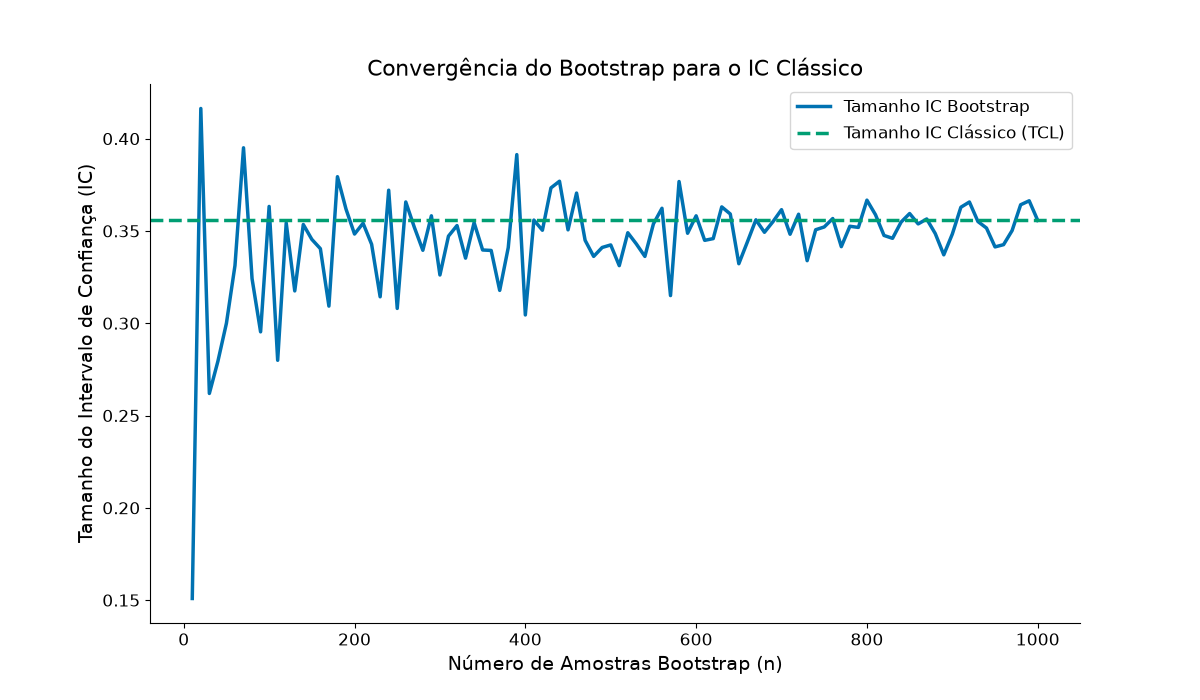
\includegraphics[width=\textwidth]{01_convergencia_sintetica.png}
        \end{column}
    \end{columns}
\end{frame}
